
%(BEGIN_QUESTION)
% Copyright 2006, Tony R. Kuphaldt, released under the Creative Commons Attribution License (v 1.0)
% This means you may do almost anything with this work of mine, so long as you give me proper credit

Det er mulig å måle nivået av et væske-væske-grensesnitt ved hjelp av en flottør:

$$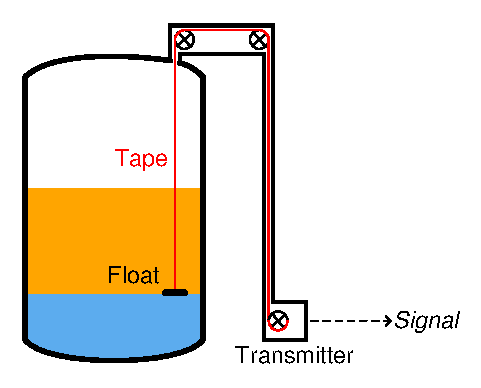
\includegraphics[width=15.5cm]{i00312x01.eps}$$

Forklar hvilke egenskaper flottøren må ha for å kunne holde seg ved grensesnittnivået.  Beskriv også noen mulige fordeler denne teknikken har sammenlignet med grensesnittmåling basert på hydrostatisk trykk.

\vskip 20pt \vbox{\hrule \hbox{\strut \vrule{} {\bf Forslag til sokratisk diskusjon} \vrule} \hrule}

\begin{itemize}
\item{} Nevn praktiske bruksområder for måling av væskegrensesnitt i industrien.
\item{} Anta at en instrumenttekniker bytter ``båndet'' i dette nivåinstrumentet og ved et uhell bruker et som er 1.5 fot kortere enn det gamle.  Hvis alt annet i instrumentet er uendret, hvordan påvirkes kalibreringen?  Ser vi nullpunktsforskyvning, spennforskyvning, linearitetsendring, eller en kombinasjon?
\end{itemize}

\underbar{file i00312}
%(END_QUESTION)





%(BEGIN_ANSWER)


%(END_ANSWER)





%(BEGIN_NOTES)

Det er ett hovedkrav til flottøren:

$$D_{fluid(light)} < D_{float} < D_{fluid(heavy)}$$

\vskip 10pt

Mulige fordeler med flottørmåling sammenlignet med hydrostatisk måling:

\begin{itemize}
\item{} Robusthet mot små endringer i væsketetthet
\item{} Ingen behov for fast væskehøyde (overløp på tanktopp)
\end{itemize}

\vskip 10pt

Vi kan lage en spesialflottør i hulmetall, og deretter fylle hulrommet med et tungt materiale (væske eller faststoff) til total ``tetthet'' blir riktig.

%INDEX% Measurement, interface level: float

%(END_NOTES)
